%iffalse
\let\negmedspace\undefined
\let\negthickspace\undefined
\documentclass[journal,12pt,onecolumn]{IEEEtran}
\usepackage{cite}
\usepackage{amsmath,amssymb,amsfonts,amsthm}
\usepackage{algorithmic}
\usepackage{graphicx}
\usepackage{textcomp}
\usepackage{xcolor}
\usepackage{txfonts}
\usepackage{listings}
\usepackage{enumitem}
\usepackage{mathtools}
\usepackage{gensymb}
\usepackage{comment}
\usepackage[breaklinks=true]{hyperref}
\usepackage{tkz-euclide} 
\usepackage{listings}
\usepackage{gvv}                                        
%\def\inputGnumericTable{}                                 
\usepackage[latin1]{inputenc}     
\usepackage{xparse}
\usepackage{color}                                            
\usepackage{array}                                            
\usepackage{longtable}                                       
\usepackage{calc}                                             
\usepackage{multirow}
\usepackage{multicol}
\usepackage{hhline}                                           
\usepackage{ifthen}                                           
\usepackage{lscape}
\usepackage{tabularx}
\usepackage{array}
\usepackage{float}
\newtheorem{theorem}{Theorem}[section]
\newtheorem{problem}{Problem}
\newtheorem{proposition}{Proposition}[section]
\newtheorem{lemma}{Lemma}[section]
\newtheorem{corollary}[theorem]{Corollary}
\newtheorem{example}{Example}[section]
\newtheorem{definition}[problem]{Definition}
\newcommand{\BEQA}{\begin{eqnarray}}
\newcommand{\EEQA}{\end{eqnarray}}
\usepackage{float}
\usepackage{listings}
\usepackage{xcolor}
%\newcommand{\define}{\stackrel{\triangle}{=}}
\theoremstyle{remark}
\usepackage{ circuitikz }
%\newtheorem{rem}{Remark}
% Marks the beginning of the document
\begin{document}
\title{9.1.5}
\author{EE24BTECH11007 - Arnav Makarand Yadnopavit}
\maketitle
\renewcommand{\thefigure}{\theenumi}
\renewcommand{\thetable}{\theenumi}
\parindent 0px Question: Solve the differential equation $\frac{d^2y}{dx^2}=\cos3x+\sin3x$ with initial conditions $y\brak{0}=0$ and $y^\prime\brak{0}=\frac{1}{3}$. \\
\solution\\
\textbf{Theoretical Solution:}\\
Integrating with respect to $x$ on both sides
\begin{align}
    \int\frac{d^2y}{dx^2}dx&=\int \cos3x+\sin3xdx \label{eq:first}\\
    \frac{dy}{dx}&=\frac{\sin3x}{3}-\frac{\cos3x}{3}+c_1    
\end{align}
Using initial condition $y^\prime\brak{0}=-\frac{1}{3}$
\begin{align}
    c_1&=0\\
    \implies\frac{dy}{dx}&=\frac{\sin3x}{3}-\frac{\cos3x}{3}\label{eq:y}\\
\end{align}
Again integrate on both sides with respect to $x$
\begin{align}
    \int \frac{dy}{dx} dx&=\int -\frac{\sin3x}{3}+\frac{\cos3x}{3} dx\\
    y&=-\frac{\cos3x}{9}-\frac{\sin3x}{9}+c_2\\
\end{align}
Using initial condition $y\brak{0}=\frac{-1}{9}$
\begin{align}
    \implies c_2&=\frac{1}{9}\\
    \therefore y&=-\frac{\cos3x}{9}-\frac{\sin3x}{9}+\frac{1}{9}
\end{align}
The theoretical solution is $f\brak{x}=-\frac{\cos3x}{9}-\frac{\sin3x}{9}+\frac{1}{9}$\\\\
\textbf{Computational Solution:}\\
Using trapezoidal rule to get difference equation
\begin{align}
    x_0&=0\\
    y_0&=0\\
    h&=0.001\\
    x_{n+1}&=x_{n}+h\\
    y_{n+1}&=y_n+\frac{h}{2}\brak{y^\prime_{n+1}+y^\prime_{n}}\\
    \implies y_{n+1}&=y_n+\frac{h}{2}\brak{\brak{-\frac{\sin3x_{n}}{3}+\frac{\cos3x_{n}}{3}}+\brak{-\frac{\sin3x_{n-1}}{3}+\frac{\cos3x_{n-1}}{3}}}
\end{align}
\textbf{Another approach} : \\
Consider \eqref{eq:y}. Let the Laplace transform of RHS be $X(s)$. Then, 
\begin{align}
	g(t) &= \frac{\sin3t}{3}-\frac{\cos3t}{3} \\
	\frac{dy}{dt} &= g(t) \label{eq:1}
\end{align}
Applying Laplace transform on both the sides of \eqref{eq:1} , we have 
\begin{align}
	s Y(s) &= X(s) 
\end{align}
The transfer function, $H(s)$ can then be defined as
\begin{align}
	H(s) &= \frac{Y(s)}{X(s)} \\
	H(s) &= \frac{1}{s} \label{eq:bil}
\end{align}
Applying \textbf{Bi-linear transform} on both sides of \eqref{eq:bil}, i.e., converting $s$-domain into $z$-domain, we have
\begin{align}
	s &= \frac{2}{h} \brak{\frac{1 - z^{-1}}{1 + z^{-1}}} \\
	H(z) &= \frac{h}{2} \brak{\frac{1 + z^{-1}}{1 - z^{-1}}} \\
	Y(z) &= \frac{h}{2} \brak{\frac{1 + z^{-1}}{1 - z^{-1}}} X(z) \\
	\brak{1 - z^{-1}} Y(z) &= \frac{h}{2} \brak{1 + z^{-1}} X(z) \label{eq:iz} 
\end{align}
Taking \textbf{Inverse z-transform} on both the sides of \eqref{eq:iz} , we have
\begin{align}
	y_{n} - y_{n-1} &= \frac{h}{2} \brak{g(x_{n}) + g(x_{n-1})} \\
	y_{n} &= y_{n-1} + \frac{h}{2} \brak{g(x_{n}) + g(x_{n-1})} \label{eq:difeq2}\\
    \implies y_{n+1}&=y_n+\frac{h}{2}\brak{\brak{-\frac{\sin3x_{n}}{3}+\frac{\cos3x_{n}}{3}}+\brak{-\frac{\sin3x_{n-1}}{3}+\frac{\cos3x_{n-1}}{3}}}
\end{align}
\begin{figure}[h]
    \centering
    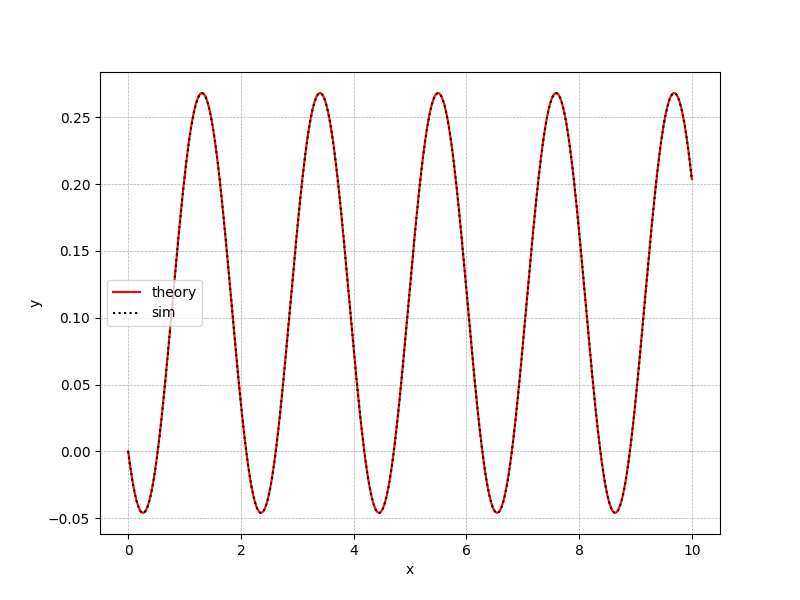
\includegraphics[width=\columnwidth]{figs/fig.png}
 \end{figure}
\end{document}
